\documentclass[titlepage]{article}

 % Dans le préambule
%\usepackage[style=author]{biblatex} % package de bibliographie, on cite l’auteur
%\addbibresource{Bib2Validation.bib} % notre fichier bib exporté

%%%%% Tous les packages
\usepackage[left=2cm,right=2cm,top=2cm,bottom=2cm]{geometry}
\usepackage[utf8]{inputenc}% accents in
\usepackage[english]{babel}% typo française
\usepackage[T1]{fontenc}% accents out
\usepackage{lmodern}
\usepackage{titlepic}
\usepackage[noae]{Sweave} % "noae" permet à Sweave de reconnaitre les guillemets
\usepackage[%
    all,
    defaultlines=3 % nombre minimum de lignes
]{nowidow} % éviter les lignes orphelines

% package maths
\usepackage{amsmath}
\usepackage{amsfonts}
\usepackage{amssymb}
\usepackage{ dsfont } %proba
\usepackage{ stmaryrd }
% tables et figures
\usepackage{longtable}
\usepackage{subfigure}
\usepackage{lscape}
\usepackage{multirow} % permet de fusionner les colonnes
\usepackage{graphicx} % admet les figures
\usepackage{array} % types particuliers de tableaux
\usepackage{tabularx} % autres tableaux, notamment pour gérer les doubles traits de séparation (voir hhline)
\usepackage{listings} % pas forcément utile ici, mais permet de faire des box avec du code
\usepackage[hang,font = normalsize, labelfont=bf,textfont=bf]{caption} % mise en forme du caption
% hyperlinks
\usepackage{hyperref}
\hypersetup{ %moduler les couleurs des liens
    colorlinks=true,
    linkcolor=black,
    % filecolor=magenta,      
    urlcolor= blue,
}
\usepackage{indentfirst} % Pour indenter les premiers paragraphes de section
%kableExtra
\usepackage{booktabs}
\usepackage{longtable}
\usepackage{array}
\usepackage{multirow}
\usepackage{wrapfig}
\usepackage{float}
\usepackage{colortbl}
\usepackage{pdflscape}
\usepackage{tabu}
\usepackage{threeparttable}
\usepackage{threeparttablex}
\usepackage[normalem]{ulem}
\usepackage{makecell}
\usepackage{xcolor}
\usepackage{hyperref} %pour les liens url
%\usepackage[absolute,overlay]{textpos}

% Pour ne pas que la mention "Chapter" apparaisse à chaque chapitre mais juste le titre du chapitre
\usepackage{titlesec}
\titleformat{\chapter}{\normalfont\LARGE}{\thechapter.}{30pt}{\LARGE\bf}
\titleformat{\section}
  {\normalfont\fontsize{15}{15}\bfseries}{\thesection}{1em}{}
\titlespacing*{\chapter}{0pt}{1.1\baselineskip}{\baselineskip}



% Ne pas sauter de page entre deux chapitres





% titres
\title{\centering 

\vspace{1 cm}

{\begin{minipage}\linewidth
        \centering
     \textbf{Un effet inattendu du confinement : une chute de la surmortalité violente chez les jeunes ?} \\[1 cm] 
        \vspace{0.5cm}
        \large Abel Aussant, Eliot Forcadell et Ariane Sessego\\
         M2 Quantifier en Sciences Sociales\\
        \vspace{0.5cm}
         \textit{Identification causale} Cours d'Olivier Godechot \\
         Année académique 2021-2022\\
    \end{minipage}}
  }
\date{}
%box

\begin{document}
\Sconcordance{concordance:Aussant_Forcadell_Sessego.tex:Aussant_Forcadell_Sessego.Rnw:%
1 116 1 1 19 31 1 1 16 3 1 1 10 1 7 55 1}

\Sconcordance{concordance:Aussant_Forcadell_Sessego.tex:Aussant_Forcadell_Sessego.Rnw:%
1 116 1 1 19 31 1 1 16 3 1 1 10 1 7 55 1}

\maketitle

\cleardoublepage%

En 2020, les épisodes de confinements ont bouleversé la vie des Français. Ces restrictions de sortie en dehors du domicile avaient pour but de protéger les plus vulnérables du virus de la Covid-19, particulièrement les personnes âgées. Mais on peut se demander s'ils n'ont pas aussi eu des effets inattendus : le confinement a-t-il entrainé une diminution de la mortalité chez les jeunes ? \\

En effet, le risque de décès entre 15 et 30 ans est souvent plus élevé que l'on ne pourrait s'y attendre face à l'augmentation exponentielle de la mortalité habituellement constatée entre 10 et 60 ans (Remund, Camarada, 2021). On désigne donc comme "surmortalité" cet excès par rapport au risque de décès attendu, qui a longtemps été considéré comme uniquement masculin, lié aux turbulences hormonales et de développement biologiques des jeunes hommes\footnote{Heligman L., Pollard J.H., The age pattern of mortality, Journal of the Institute of Actuaries, 1980, 107(1), p. 49-80 et  Goldstein J. A., Secular trend toward earlier male sexual maturity: Evidence from shifting ages of male young adult mortality, PLoS ONE, 2011, 6(8), e14826.}, et liée à des causes violentes de décès (accidents, homicides...). Ces théories développementalistes ont été largement remises en question, du fait des variations de cette tendance dans le temps et l'espace ; on considère aujourd'hui cette surmortalité comme avant tout liée à des contextes socio-historiques particuliers (Remund, Camarada, 2021). En France aujourd'hui, bien qu'elle touche aussi les jeunes femmes, cette surmortalité est bien plus importante parmi les hommes, avec en moyenne trois fois plus de décès masculins que féminin à ces âges (Breton, Barbieri, 2018), même si cette écart à tendance à se réduire. Elle est avant tout caractérisée par une part importante de morts violentes (accidents, homicides ou suicides) qui sont l'origine de 80\% des décès à ces âges, tout particulièrement les accidents de la circulation (Remund, Camarada, 2021). \\

Le confinement a théoriquement réduit l'exposition à ces risques, à l'exception du suicide. A-t-il entraîné une diminution de la mortalité au sein de cette population ? Le deuxième confinement, moins restrictif que le premier, a-t-il eu un impact plus faible sur cette mortalité ? \\

La méthode de différence de différence (DD) nous offre la possibilité de comparer la mortalité des jeunes adultes avant et pendant les périodes de confinement en prenant en compte la saisonnalité de la mortalité et une éventuelle variation de mortalité propre à 2020. En effet, il s'agit ici d'évaluer l'effet d'un "traitement" - le confinement généralisé de la population - sur un groupe traité - les jeunes adultes. En l'absence d'expérience aléatoire, nous ne disposons pas de groupe contrôle; et comme toute la population étant supposée confinée, il semble difficile d'en construire un. Mais nous pouvons procéder autrement pour construire un contrefactuel, notamment en considérant les périodes précédentes. Cela suppose cependant que l’évolution de la mortalité dans la population cible (les jeunes adultes) est comparable entre période. Or, on sait que la mortalité connait des tendances saisonnières importantes : la mortalité des jeunes adultes, en particulier, connait deux pics annuels, un plus faible en hiver (en février particulièrement), qui suit la tendance générale de la population, l'autre plus important en été (en juillet), qui est lié à une augmentation estivale de mortalité par accidents (Breton, 2019). Ces tendances nous empêche de comparer simplement la période pré-confinement à la période de confinement. La DD nous permet, en supposant que l'évolution de la mortalité est comparable d'une année sur l'autre, de comparer la mortalité en 2020 (groupe traité) et pendant les années précédentes (groupe contrôle), avant les confinements (période précédent le traitement) et durant chaque confinement (période de traitement), afin de mettre en avant un eventuel effet causal du confinement sur la mortalité des jeunes adultes. \\

Après une présentation des données et quelques analyses descriptives, nous présenterons en détail les modèles choisis, pour ensuite commenter les résultats.


\section*{Données et méthode}



\subsubsection*{Les décès d'individus de 18 à 29 ans par date, en France métropolitaine, de 2014 à 2020}

Pour répondre à ces questions, nous utilisons les données d'état civil mises à disposition par l'INSEE, répertoriant les personnes décédées par date de décès, année de naissance, sexe, et lieu de décès pour les années 2014 à 2020 (INSEE 2014 à 2020, voir Sources, \textit{infra}). Nous disposons du jour, du mois et de l'année de décès pour 2018 à 2020, mais uniquement du mois et de l'année de décès pour 2014 à 2017. \\

Nous considérons ici les décès d'individus âgés de 18 à 29 ans (age révolu au moment du décès), afin de prendre en compte cette population de jeunes adultes en âge de conduire, les accidents de la circulation étant parmi les premières causes de décès chez les jeunes (INSERM, 2020) et le risque qui aurait le plus diminué durant le confinement. Nous avons de plus fait le choix de ne considérer que les décès survenus en France métropolitaine, d'une part car la littérature concernant les Outre-mer est plus rare et il est fort probable que la mortalité ne suive pas les mêmes tendance, étant donné la différence des saisons et des périodes de congé, et d'autre part car l'application du confinement, particulièrement pour le deuxième, y a été différente. \\

%Nous pouvons ici considérer le nombre de décès journaliers (en imputant une moyenne par jour pour les années précédent 2018) en considérant 

Nous raisonnerons ici par nombre de décès bruts, et non par taux de mortalité, car cela nécessiterait de rapporter ces décès brut à la taille de la population des jeunes adultes sur chaque période. En effet, d’après l’INSEE, de 2014 à 2020, la population des 18-29 ans a évolué de 9,4 millions à 9,3 millions (INSEE, 2022), une variation de l’ordre de 0,1\%, que l'on peut considérer comme négligeable. De plus, le raisonnement en nombre de décès permet de conserver un ordre de grandeur familier et directement interprétable par les non-démographes. \\ % Enfin, cette évolution tend vers une légère diminution du nombre de jeunes de 18 à 29 ans, ce qui tendrait à diminuer le nombre de décès

Les périodes de confinement que nous considérons sont les suivantes : ...

\subsubsection*{Une faible mortalité absolue des jeunes adultes rendant plus difficile l'identification d'une tendance}

De 2014 à 2020, au total 25 481 jeunes adultes de 18 à 29 ans sont décédés en France métropolitaine, avec un effectif de décès par année stable de l'ordre de 3 600 décès. En moyenne, il y 10 décès par jour sur toute la période avec une légère baisse de cette moyenne en 2019 (9,9 décès par jour) et 2020 (9,7 décès par jour), mais qu'il est difficile d'interpréter pour le moment. L'écart-type des décès par jour est également plutôt stable en fonction de la période considérée, allant de 3.3 à 3.5. L'écart-type de 2.3 indiqué sur l'ensemble de la période est artificiellement bas puisque nous imputons à chaque jour le nombre de décès de ce mois mois divisé par le nombre de jour dans ce mois, réduisant artificiellement la variation des décès par jour. Il n'est donc pas possible de tirer de conclusion à partir de ce chiffre. \\

\begin{table}[!h]

\caption{\label{tab:Descr}Statistiques descriptives du nombre de décès journalier des 18 à 29 ans}
\centering
\begin{threeparttable}
\begin{tabular}[t]{lrrrrrr}
\toprule
  & Effectif total sur la période & Moyenne & Médiane & Ecart-type & Maximum & Minimum\\
\midrule
2014-2020* & 25481 & 10.0 & 10 & 2.3 & 23 & 0\\
2018-2019 & 7269 & 10.0 & 10 & 3.4 & 23 & 1\\
2018 & 3643 & 10.0 & 10 & 3.3 & 23 & 1\\
2019 & 3626 & 9.9 & 10 & 3.5 & 23 & 2\\
2020 & 3538 & 9.7 & 9 & 3.4 & 20 & 0\\
\bottomrule
\end{tabular}
\begin{tablenotes}
\small
\item *Pour 2014 à 2017, comme nous disposons que du mois de décès, nous avons imputé un n-ème du nombre de décès par mois, avec n le nombre de jours dans le mois.
\item Source : INSEE, 2014 à 2020.
\item Champ : Décès de personnes agées de 18 à 29 ans survenus en France métropolitaine de 2014 à 2020.
\item Lecture : En 2020, 3 538 jeunes adultes âgés de 18 à 29 ans sont décédés, avec une moyenne de 9,7 décès par jours, et un écart-type de décès par jours de 3,4. Au cours de l'année, il y a eu au maximum 20 décès de jeunes adultes et au minimum aucun décès survenus en un jour.
\end{tablenotes}
\end{threeparttable}
\end{table}
On peut tout d'abord souligner que ces effectifs journaliers de décès sont faibles, du fait de la faible mortalité des jeunes adultes, ce qui est - dans l'absolu - réjouissant. Cependant, le nombre de décès étant nécessairement un entier, cela implique des variations importantes, rendant difficile l'identification d'une tendance. Or, la DD repose sur le postula qu'il y ait une évolution identique de la variable d'intérêt - ici le nombre de décès des jeunes adultes - dans les deux groupes avant le traitement (2020 avant le confinement et les années précédentes), ce que l'on souhaiterait pouvoir apprécier avant d'estimer les modèles. \\

Les Figures \ref{fig:courbe_2018_2019} et \ref{} cherchent à dégager ces évolutions et les comparer aux tendances pendant les confinements. Les lignes grises sur la Figure 1 représentant les évolutions brutes du nombre de décès par jour pour les années 2018 à 2020 montre à quel point il est difficile d'en dégager les tendances sans une analyse plus poussée. Nous avons donc procédé à un lissage des tendances par l'intermédiaire de la méthode des fenêtres gaussiennes. Chaque point de la courbe lissé est estimé en fonction d'une pondération des fréquences observée de part et d'autre du point, par l'intermédiaire de coefficients estimés par l'intermédiaire d'une fonction gaussienne calculée sur un fenêtre de temps déterminée\footnote{Pour le détail de la méthode voir : \url{https://au.mathworks.com/help/signal/ref/gausswin.html}, les paramètres utilisés ici sont : }. \textit{EEEeuuuh, je n'ai aucune idée si cette phrase a du sens, mais j'ai l'impression de me comprendre}. Ce lissage nous laisse entrevoir une certaine diminution du nombre décès au cours de la période du premier confinement, par rapport aux années 2018 et 2019. Cependant, mais il est difficile d'interpréter les courbes car on peut encore percevoir la très forte volatilité du nombre de décès. Les tendances pré-confinement ne coïncident pas entièrement de 2018 à 2020, avec en particulier une légère augmentation en 2020 juste avant le premier confinement qui pourrait apparaitre comme une surmortalité par rapport aux deux années précédentes. Serait-ce dû à une surmortalité due à la Covid-19? Cela semble très peu probable étant donné que les formes graves de la maladie ont très peu touchées les jeunes adultes. Il semble difficile d'apprécier ici la moindre différence ou convergence car les variations demeurent faibles (en dessous d'un peu moins de deux écart-types). \\

\begin{figure}
\begin{center}
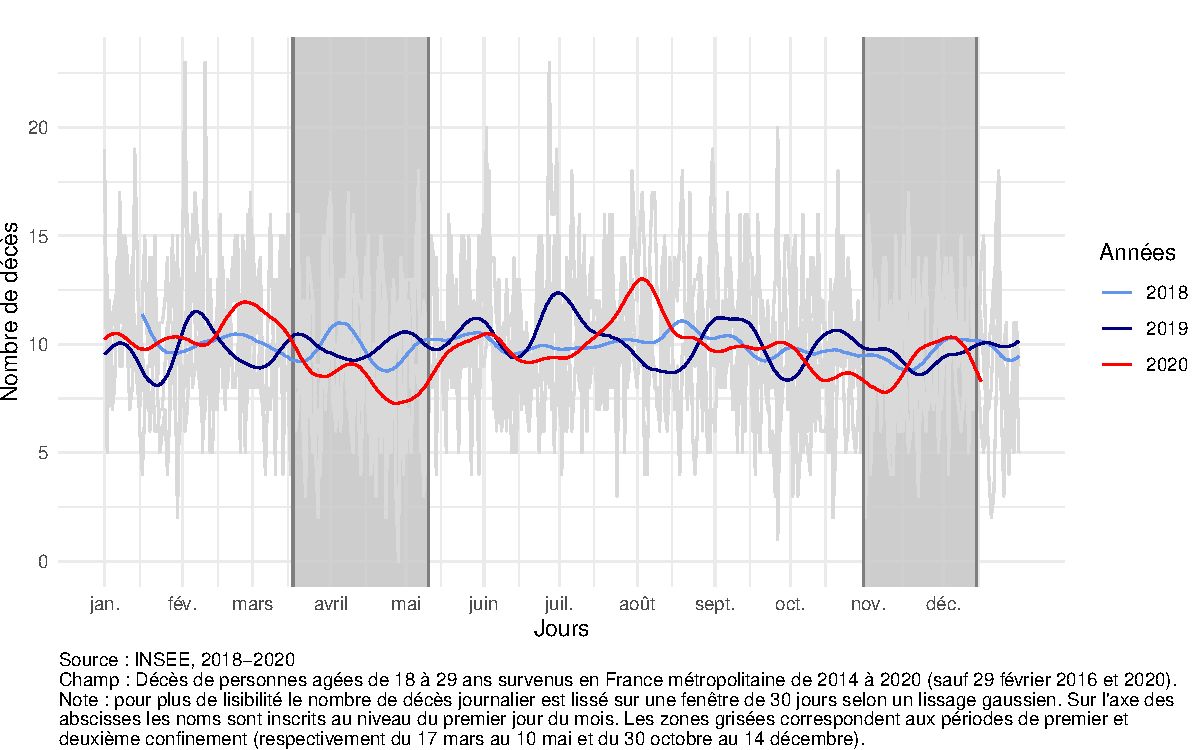
\includegraphics{Aussant_Forcadell_Sessego-courbe_2018_2019}
\end{center}
\end{figure}

\begin{figure}
\begin{center}
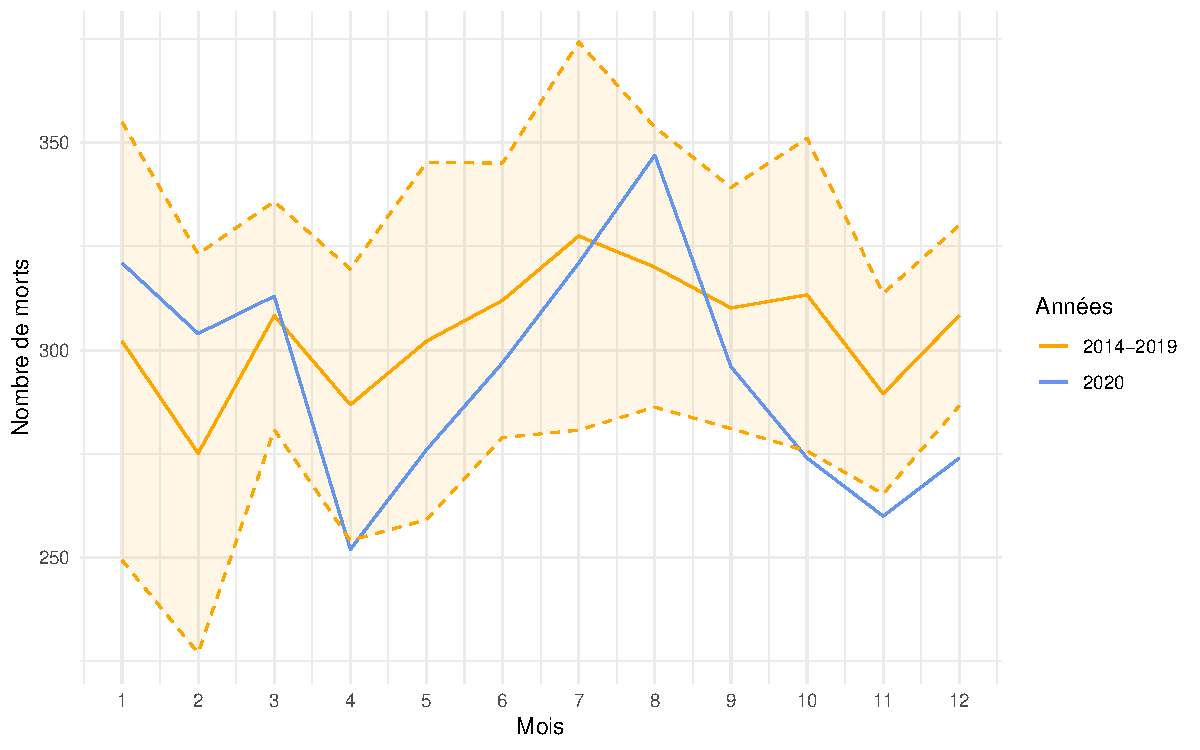
\includegraphics{Aussant_Forcadell_Sessego-courbe_2014_2020}
\end{center}
\end{figure}

% Ne pas oublier de mentionner quelque part que l'on supprime le 29 février de l'analyse

Cela peut s'expliquer par nombreux biais conjoncturels qui peuvent avoir une influence sur la mortalité mais surtout un aléa important car les effectifs des décès parmi les jeunes adultes sont si faibles. C'est ce qui nous a inviter à introduire les années 2014 à 2017 dans la comparaison, bien que nous ne disposons pas du jour exact de décès La Figure 2 présente le nombre de décès par mois en 2020 par rapport à la moyenne des décès par mois de 2014 à 2019 et un intervalle de confiance à 90\%, afin de mettre en évidence une éventuelle tendance sous-jacente au nombre de décès de jeunes adultes par mois. \\

L'on retrouve ici des résultats démontrés dans la littérature : deux pics annuels de mortalité parmi les jeunes, l'un plus faible en hiver (entre janvier et mars sur notre graphique) et l'autre plus important en été (en juillet) (Breton, 2019). L'intervalle de confiance demeure important, cependant le nombre de décès au cours des mois d'avril et de novembre-décembre en 2020 ce situent en dehors de celui-ci, ce qui semble confirmer notre hypothèse d'une réduction de la mortalité des jeunes adultes au court des périodes de confinement par rapport aux années précédentes. De plus, la tendance observées pour janvier, février et mars 2020 suivent de manière convaincantes celle des années 2014 à 2019, tendant à conforter l'idée d'une évolution identique de la mortalité entre année avant la survenue du confinement. \\

Cependant, en comparant l'évolution du nombre de décès entre mai et septembre pour l'année 2020 par rapport aux années 2014 à 2019, on peut se demander si le confinement ne pourrait pas avoir eu l'effet inverse que celui attendu après la fin des restrictions. En effet, on observe dans la Figure 2, tout comme dans la Figure 3, une augmentation du nombre de décès de mai à août. On peut en effet supposer que les restrictions imposées lors du confinement, bien qu'elles aient pu avoir un effet protecteur pour les jeunes adultes lors du confinement, ont pu occasionner un effet rebond au cours de la période estivale qui a suivi, où l'intensité des activités à repris de plus belles pour compenser les restrictions des mois précédents. Ainsi, si le confinement a permis de sauver des vies, le même nombre de vie n'a-t-il pas été perdu au court de l'été qui a suivi ? Quel effet du confinement sur le long terme ? \\

\textit{Je n'arrive pas à changer la taille des figures... Je ne sais pas pourquoi, mais je pense que ça devrait être réglable, pour les faire rentrer sur toute la largeur de la page}



\section*{Modèles et résultats}

\subsubsection*{Les modèles de régressions choisies}

Nous chercherons à répondre à ces questions par l'intermédiaire des modèles suivants.


\section*{Conclusion (et Discussion?)}






\section*{Sources} \label{source}

\begin{itemize}
\item INSEE, 2022, \url{https://www.insee.fr/fr/outil-interactif/5014911/pyramide.htm#!y=2015&a=18,30&v=2&c=0}

\item INSEE, 2020, \url{https://www.insee.fr/fr/statistiques/5431034?sommaire=5419788&q=d\%C3\%A9c\%C3\%A8s+2020}
\item INSEE, 2019, \url{https://www.insee.fr/fr/statistiques/4801913?sommaire=4768339&q=d\%C3\%A9c\%C3\%A8s+2019}
\item INSEE, 2018, \url{https://www.insee.fr/fr/statistiques/4216603?sommaire=4215184}
\item INSEE, 2017, \url{https://www.insee.fr/fr/statistiques/3606190?sommaire=3596198}
\item INSEE, 2016, \url{https://www.insee.fr/fr/statistiques/3053349?sommaire=3051496}
\item INSEE, 2015, \url{https://www.insee.fr/fr/statistiques/2406453?sommaire=2406457}
\item INSEE, 2014, \url{https://www.insee.fr/fr/statistiques/2114975?sommaire=2114983}

\item INSERM, 2020 \url{http://cepidc-data.inserm.fr/inserm/html/index2.htm}
\end{itemize}


\end{document}
